\documentclass[11pt,a4paper]{article}

% Packages
\usepackage[utf8]{inputenc}
\usepackage[T1]{fontenc}
\usepackage{geometry}
\usepackage{graphicx}
\usepackage{xcolor}
\usepackage{fancyhdr}
\usepackage{titlesec}
\usepackage{booktabs}
\usepackage{longtable}
\usepackage{multirow}
\usepackage{array}
\usepackage{enumitem}
\usepackage{amsmath}
\usepackage{siunitx}
\usepackage{hyperref}
\usepackage{tcolorbox}
\usepackage{tikz}
\usepackage{pgfplots}
\usepackage{background}
\usepackage{lipsum}

\pgfplotsset{compat=1.18}
\usetikzlibrary{shapes,arrows,positioning,calc}

% Page geometry
\geometry{
    a4paper,
    left=25mm,
    right=25mm,
    top=30mm,
    bottom=30mm,
    headheight=15pt
}

% Colors
\definecolor{primaryblue}{RGB}{102,126,234}
\definecolor{secondarypurple}{RGB}{118,75,162}
\definecolor{accentorange}{RGB}{249,115,22}
\definecolor{darkgray}{RGB}{51,51,51}
\definecolor{lightgray}{RGB}{245,245,245}

% Hyperref setup
\hypersetup{
    colorlinks=true,
    linkcolor=primaryblue,
    filecolor=secondarypurple,
    urlcolor=primaryblue,
    citecolor=primaryblue,
    pdfauthor={C. Nicholls},
    pdftitle={R50k Solar PV + BESS Solution - Engineering Design},
    pdfsubject={Solar Energy System Design},
    pdfkeywords={Solar, PV, Battery, Energy Storage, Huawei}
}

% Header and Footer
\pagestyle{fancy}
\fancyhf{}
\fancyhead[L]{\small\textcolor{primaryblue}{UtCS (Pty) Ltd}}
\fancyhead[R]{\small\textcolor{gray}{CONFIDENTIAL}}
\fancyfoot[L]{\small Eng. C. Nicholls}
\fancyfoot[C]{\small\thepage}
\fancyfoot[R]{\small\today}
\renewcommand{\headrulewidth}{0.5pt}
\renewcommand{\footrulewidth}{0.5pt}

% Title formatting
\titleformat{\section}
{\color{primaryblue}\Large\bfseries}
{\thesection}{1em}{}[\titlerule]

\titleformat{\subsection}
{\color{secondarypurple}\large\bfseries}
{\thesubsection}{1em}{}

% Custom commands
\newcommand{\highlight}[1]{\textcolor{primaryblue}{\textbf{#1}}}
\newcommand{\money}[1]{\textbf{R\,#1}}

\begin{document}

% Title Page
\begin{titlepage}
    \begin{center}
        \vspace*{2cm}
        
        % Watermark
        
\begin{tikzpicture}[remember picture,overlay]
            \node[opacity=0.1,scale=3] at (current page.center) {\Huge\textbf{CONFIDENTIAL}};
        \end{tikzpicture}
        
        {\Huge\bfseries\color{primaryblue} R50,000 Solar PV + BESS Solution}
        
        \vspace{0.5cm}
        
        {\Large\color{secondarypurple} 15-20 kWh Daily Base Load Capacity}
        
        \vspace{1cm}
        
        {\large Professional Engineering Design Document}
        
        \vspace{2cm}
        
        \begin{tcolorbox}[colback=lightgray,colframe=primaryblue,width=0.8\textwidth,arc=3mm]
            \centering
            \textbf{Project Reference:} UTCS-SOLAR-2026-001 \\
            \vspace{0.3cm}
            \textbf{Client:} [Client Name] \\
            \vspace{0.3cm}
            \textbf{Location:} [Installation Address] \\
            \vspace{0.3cm}
            \textbf{Date:} \today
        \end{tcolorbox}
        
        \vfill
        
        \begin{minipage}{0.4\textwidth}
            \begin{flushleft}
                \textbf{Prepared by:} \\
                C. Nicholls \\
                Professional Engineer \\
                UtCS (Pty) Ltd
            \end{flushleft}
        \end{minipage}
        \hfill
        \begin{minipage}{0.4\textwidth}
            \begin{flushright}
                \textbf{Classification:} \\
                \textcolor{red}{\textbf{CONFIDENTIAL}} \\
                For Authorized Use Only
            \end{flushright}
        \end{minipage}
        
        \vspace{1cm}
        
        \hrule
        \vspace{0.3cm}
        {\small UtCS (Pty) Ltd | Renewable Energy Solutions | www.utcs.co.za}
        
    \end{center}
\end{titlepage}

% Table of Contents
\tableofcontents
\newpage

% Executive Summary
\section{Executive Summary}

This document presents a comprehensive engineering design for a \money{50,000} (including VAT) solar photovoltaic (PV) system with battery energy storage (BESS), designed to provide 15-20 kWh of daily base load electricity for residential applications.

\subsection{Key Highlights}

\begin{tcolorbox}[colback=lightgray,colframe=primaryblue,title=Project Overview]
\begin{itemize}[leftmargin=*]
    \item \textbf{Total Investment:} \money{49,892.75} (incl. VAT) - \textcolor{green!60!black}{0.2\% under budget}
    \item \textbf{PV Capacity:} 2.75 kW (5 × 550W monocrystalline panels)
    \item \textbf{Battery Storage:} 10.24 kWh total (9.22 kWh usable @ 90\% DoD)
    \item \textbf{Daily Energy Capacity:} 18.5 kWh/day (PV + Battery)
    \item \textbf{Target Load Support:} 15.0 kWh/day (within 15-20 kWh specification)
    \item \textbf{System Type:} Grid-tied hybrid with battery backup
    \item \textbf{Compliance:} NRS 097-2-1:2017, SANS 10142-1:2017
\end{itemize}
\end{tcolorbox}

\subsection{System Performance}

The designed system provides reliable renewable energy generation with the following performance characteristics:

\begin{table}[h]
\centering
\begin{tabular}{@{}lcc@{}}
\toprule
\textbf{Parameter} & \textbf{Value} & \textbf{Unit} \\
\midrule
Daily PV Generation & 9.28 & kWh/day \\
Battery Usable Capacity & 9.22 & kWh \\
Total Daily Capacity & 18.5 & kWh/day \\
System Efficiency & 75 & \% \\
Self-Consumption Rate & 85 & \% \\
Peak Sun Hours (Average) & 4.5 & hours \\
\bottomrule
\end{tabular}
\caption{System Performance Summary}
\end{table}

\newpage

\section{System Design Specifications}

\subsection{Photovoltaic (PV) Array}

The PV array consists of high-efficiency monocrystalline panels optimized for South African solar irradiance conditions.

\begin{tcolorbox}[colback=blue!5,colframe=primaryblue,title=PV Array Specifications]
\begin{itemize}[leftmargin=*]
    \item \textbf{Total Capacity:} 2.75 kW\textsubscript{p}
    \item \textbf{Panel Quantity:} 5 panels
    \item \textbf{Panel Model:} JA Solar JAM72S30-550W
    \item \textbf{Panel Type:} Monocrystalline PERC
    \item \textbf{Panel Efficiency:} 21.3\%
    \item \textbf{Panel Dimensions:} 2278 × 1134 × 35 mm
    \item \textbf{Performance Warranty:} 25 years (80\% at year 25)
    \item \textbf{Product Warranty:} 12 years
    \item \textbf{Expected Daily Generation:} 9.28 kWh (at 4.5 peak sun hours, 75\% system efficiency)
\end{itemize}
\end{tcolorbox}

\subsubsection{PV Array Configuration}

The panels will be configured in a single string connected to the hybrid inverter's MPPT input:

\begin{itemize}
    \item \textbf{String Configuration:} 5 panels in series
    \item \textbf{String Voltage (V\textsubscript{oc}):} Approximately 230V DC
    \item \textbf{String Current (I\textsubscript{sc}):} Approximately 14A DC
    \item \textbf{Mounting:} Roof-mounted on aluminum rails at optimal tilt angle
\end{itemize}

\subsection{Hybrid Inverter}

The system utilizes a Huawei hybrid string inverter with integrated battery management capabilities.

\begin{tcolorbox}[colback=green!5,colframe=green!60!black,title=Inverter Specifications]
\begin{itemize}[leftmargin=*]
    \item \textbf{Model:} Huawei SUN2000-3KTL-L1
    \item \textbf{Rated Power:} 3 kW
    \item \textbf{Type:} Hybrid String Inverter
    \item \textbf{Maximum Efficiency:} 98.3\%
    \item \textbf{MPPT Trackers:} 2 independent trackers
    \item \textbf{Input Voltage Range:} 90-560V DC
    \item \textbf{Output:} Single Phase, 230V AC, 50Hz
    \item \textbf{Protection:} IP65 rated enclosure
    \item \textbf{Communication:} WiFi, RS485, Smart Dongle
    \item \textbf{Monitoring:} Huawei FusionSolar App
    \item \textbf{Warranty:} 10 years standard
\end{itemize}
\end{tcolorbox}

\subsection{Battery Energy Storage System (BESS)}

The BESS utilizes Lithium Iron Phosphate (LiFePO4) technology for safe, long-life energy storage.

\begin{tcolorbox}[colback=orange!5,colframe=accentorange,title=Battery Storage Specifications]
\begin{itemize}[leftmargin=*]
    \item \textbf{Model:} Huawei LUNA2000-5-S0
    \item \textbf{Number of Modules:} 2 × 5.12 kWh
    \item \textbf{Total Capacity:} 10.24 kWh
    \item \textbf{Usable Capacity:} 9.22 kWh (90\% Depth of Discharge)
    \item \textbf{Battery Chemistry:} Lithium Iron Phosphate (LiFePO4)
    \item \textbf{Cycle Life:} 6,000 cycles @ 90\% DoD
    \item \textbf{Operating Voltage:} 160-560V DC
    \item \textbf{Maximum Charge/Discharge:} 2.5 kW
    \item \textbf{Efficiency:} >95\% round-trip
    \item \textbf{Operating Temperature:} -10°C to +55°C
    \item \textbf{Protection:} IP65, Active Safety Management
    \item \textbf{Warranty:} 10 years
\end{itemize}
\end{tcolorbox}

\subsection{Smart Metering}

\begin{tcolorbox}[colback=purple!5,colframe=secondarypurple,title=Smart Meter Specifications]
\begin{itemize}[leftmargin=*]
    \item \textbf{Model:} Landis+Gyr E460
    \item \textbf{Type:} 4-Quadrant Bi-Directional Smart Meter
    \item \textbf{Phase:} Single Phase
    \item \textbf{Accuracy Class:} Class 1 (IEC 62053-21)
    \item \textbf{Measurement:} Active \& Reactive Energy (Import/Export)
    \item \textbf{Communication:} RS485, Modbus RTU
    \item \textbf{Display:} LCD with backlight
    \item \textbf{Function:} Grid import/export monitoring, load profiling
\end{itemize}
\end{tcolorbox}

\subsection{Monitoring \& Security}

\subsubsection{WiFi Router}
\begin{itemize}
    \item \textbf{Model:} TP-Link Industrial WiFi Router
    \item \textbf{Rating:} Outdoor rated, IP65
    \item \textbf{Function:} Provides network connectivity for inverter monitoring and CCTV
\end{itemize}

\subsubsection{CCTV Camera}
\begin{itemize}
    \item \textbf{Type:} WiFi CCTV Camera, 2MP resolution
    \item \textbf{Features:} Night vision, motion detection
    \item \textbf{Function:} Visual monitoring of inverter and battery system
    \item \textbf{Connectivity:} WiFi network connection
\end{itemize}

\newpage

\section{Detailed Cost Breakdown}

\subsection{Investment Summary}

\begin{table}[h]
\centering
\begin{tabular}{@{}lr@{}}
\toprule
\textbf{Category} & \textbf{Amount (ZAR)} \\
\midrule
Major Equipment (CAPEX) & 26,850.00 \\
Support Equipment \& Monitoring & 7,385.00 \\
Installation \& Labor & 7,020.00 \\
Professional Services \& Compliance & 2,130.00 \\
\midrule
\textbf{Subtotal (excl. VAT)} & \textbf{43,385.00} \\
VAT (15\%) & 6,507.75 \\
\midrule
\textbf{GRAND TOTAL (incl. VAT)} & \textbf{49,892.75} \\
\bottomrule
\end{tabular}
\caption{Investment Summary}
\end{table}

\subsection{Major Equipment (CAPEX)}

\begin{longtable}{@{}p{8cm}rrr@{}}
\toprule
\textbf{Description} & \textbf{Qty} & \textbf{Unit Price} & \textbf{Total} \\
\midrule
\endfirsthead
\toprule
\textbf{Description} & \textbf{Qty} & \textbf{Unit Price} & \textbf{Total} \\
\midrule
\endhead
5× 550W JA Solar Monocrystalline Panels & 5 & R\,1,520.00 & R\,7,600.00 \\
Huawei SUN2000-3KTL-L1 3kW Hybrid Inverter & 1 & R\,8,300.00 & R\,8,300.00 \\
2× Huawei LUNA2000 5.12kWh Battery Modules & 2 & R\,4,200.00 & R\,8,400.00 \\
Landis+Gyr E460 Smart Meter & 1 & R\,2,550.00 & R\,2,550.00 \\
\midrule
\multicolumn{3}{r}{\textbf{CAPEX Total:}} & \textbf{R\,26,850.00} \\
\bottomrule
\caption{Major Equipment Costs}
\end{longtable}

\subsection{Support Equipment \& Monitoring}

\begin{longtable}{@{}p{8cm}rrr@{}}
\toprule
\textbf{Description} & \textbf{Qty} & \textbf{Unit Price} & \textbf{Total} \\
\midrule
\endfirsthead
\toprule
\textbf{Description} & \textbf{Qty} & \textbf{Unit Price} & \textbf{Total} \\
\midrule
\endhead
TP-Link WiFi Router (Outdoor Rated) & 1 & R\,620.00 & R\,620.00 \\
WiFi CCTV Camera 2MP & 1 & R\,880.00 & R\,880.00 \\
Aluminum Mounting Rails \& Clamps (5 panels) & 5 & R\,330.00 & R\,1,650.00 \\
AC/DC Surge Protection, Isolator, Breaker & 1 & R\,1,650.00 & R\,1,650.00 \\
Solar DC Cable 4mm² (15m), AC Cable 4mm² (12m) & 27 & R\,35.00 & R\,945.00 \\
MC4 Connectors, Cable Glands, Terminals & 1 & R\,420.00 & R\,420.00 \\
Earthing Kit (Rods, Clamps, Earth Cable) & 1 & R\,580.00 & R\,580.00 \\
PVC Conduit 25mm \& Fittings (10m) & 10 & R\,26.00 & R\,260.00 \\
Weatherproof Enclosure (IP55) & 1 & R\,380.00 & R\,380.00 \\
\midrule
\multicolumn{3}{r}{\textbf{Support Equipment Total:}} & \textbf{R\,7,385.00} \\
\bottomrule
\caption{Support Equipment \& Monitoring Costs}
\end{longtable}

\subsection{Installation \& Labor}

\begin{longtable}{@{}p{8cm}rrr@{}}
\toprule
\textbf{Description} & \textbf{Qty} & \textbf{Unit Price} & \textbf{Total} \\
\midrule
\endfirsthead
\toprule
\textbf{Description} & \textbf{Qty} & \textbf{Unit Price} & \textbf{Total} \\
\midrule
\endhead
PV Panel Installation \& DC Wiring (5 panels) & 5 & R\,250.00 & R\,1,250.00 \\
Inverter \& Battery Installation, Configuration & 1 & R\,1,500.00 & R\,1,500.00 \\
DB Board Modifications, AC Wiring, Testing & 1 & R\,1,800.00 & R\,1,800.00 \\
E460 Smart Meter Installation \& Config & 1 & R\,750.00 & R\,750.00 \\
CCTV Camera Installation \& WiFi Setup & 1 & R\,520.00 & R\,520.00 \\
WiFi Router \& Network Configuration & 1 & R\,350.00 & R\,350.00 \\
System Testing, Commissioning \& Training & 1 & R\,850.00 & R\,850.00 \\
\midrule
\multicolumn{3}{r}{\textbf{Installation Total:}} & \textbf{R\,7,020.00} \\
\bottomrule
\caption{Installation \& Labor Costs}
\end{longtable}

\subsection{Professional Services \& Compliance}

\begin{longtable}{@{}p{8cm}rrr@{}}
\toprule
\textbf{Description} & \textbf{Qty} & \textbf{Unit Price} & \textbf{Total} \\
\midrule
\endfirsthead
\toprule
\textbf{Description} & \textbf{Qty} & \textbf{Unit Price} & \textbf{Total} \\
\midrule
\endhead
Electrical Design \& Single-Line Diagram & 1 & R\,1,000.00 & R\,1,000.00 \\
Certificate of Compliance (CoC) & 1 & R\,750.00 & R\,750.00 \\
As-Built Drawings \& O\&M Manual & 1 & R\,380.00 & R\,380.00 \\
\midrule
\multicolumn{3}{r}{\textbf{Professional Services Total:}} & \textbf{R\,2,130.00} \\
\bottomrule
\caption{Professional Services \& Compliance Costs}
\end{longtable}

\newpage

\section{System Performance Analysis}

\subsection{Energy Generation Profile}

The system's energy generation is calculated based on South African solar irradiance data:

\begin{equation}
E_{daily} = P_{PV} \times PSH \times \eta_{system}
\end{equation}

Where:
\begin{itemize}
    \item $E_{daily}$ = Daily energy generation (kWh/day)
    \item $P_{PV}$ = PV array capacity (2.75 kW)
    \item $PSH$ = Peak sun hours (4.5 hours average for SA)
    \item $\eta_{system}$ = System efficiency (0.75 or 75\%)
\end{itemize}

\begin{equation}
E_{daily} = 2.75 \times 4.5 \times 0.75 = 9.28 \text{ kWh/day}
\end{equation}

\subsection{Load Support Capability}

The system provides energy through two sources:

\begin{enumerate}
    \item \textbf{Direct PV Generation:} 9.28 kWh/day (daytime)
    \item \textbf{Battery Storage:} 9.22 kWh usable (day/night)
    \item \textbf{Total Daily Capacity:} 18.5 kWh/day
\end{enumerate}

This exceeds the target specification of 15-20 kWh/day base load support.

\subsection{System Efficiency Factors}

\begin{table}[h]
\centering
\begin{tabular}{@{}lc@{}}
\toprule
\textbf{Loss Factor} & \textbf{Efficiency} \\
\midrule
PV Panel Temperature Losses & 90\% \\
Inverter Conversion Losses & 98.3\% \\
DC Cable Losses & 98\% \\
AC Cable Losses & 99\% \\
Soiling \& Shading Losses & 95\% \\
MPPT Tracking Losses & 99\% \\
\midrule
\textbf{Overall System Efficiency} & \textbf{75\%} \\
\bottomrule
\end{tabular}
\caption{System Efficiency Breakdown}
\end{table}

\newpage

\section{Compliance \& Standards}

\subsection{South African Regulations}

This installation complies with all relevant South African electrical and renewable energy regulations:

\subsubsection{NRS 097-2-1:2017}
Grid connection code for renewable power plants connected to the electricity distribution or transmission systems. This standard covers:
\begin{itemize}
    \item Grid connection requirements
    \item Power quality standards
    \item Protection relay settings
    \item Anti-islanding protection
    \item Grid code compliance testing
\end{itemize}

\subsubsection{SANS 10142-1:2017}
The wiring of premises - Part 1: Low-voltage installations. Compliance includes:
\begin{itemize}
    \item Electrical installation safety
    \item Conductor sizing and protection
    \item Earthing and bonding requirements
    \item Switchgear and distribution boards
    \item Isolation and switching
\end{itemize}

\subsection{Certificate of Compliance (CoC)}

A Certificate of Compliance will be issued upon completion of the installation by a registered electrician, certifying that:
\begin{itemize}
    \item All electrical work complies with SANS 10142-1
    \item The installation is safe for operation
    \item All protective devices are correctly rated
    \item Earthing system meets requirements
    \item Testing and commissioning completed successfully
\end{itemize}

\subsection{Safety Features}

\begin{tcolorbox}[colback=red!5,colframe=red!60!black,title=Safety \& Protection Systems]
\begin{itemize}[leftmargin=*]
    \item \textbf{AC Surge Protection:} Type 2 SPD on AC output
    \item \textbf{DC Surge Protection:} Type 2 SPD on PV array input
    \item \textbf{DC Isolator:} Manual disconnect for PV array
    \item \textbf{AC Circuit Breaker:} 63A MCB for AC disconnect
    \item \textbf{Residual Current Device (RCD):} 30mA protection
    \item \textbf{Earthing System:} TN-S earthing with dedicated earth rods
    \item \textbf{Anti-Islanding:} Built-in inverter protection
    \item \textbf{Battery Management System (BMS):} Active cell balancing, over-voltage/under-voltage protection
    \item \textbf{Temperature Monitoring:} Automatic shutdown on over-temperature
\end{itemize}
\end{tcolorbox}

\newpage

\section{Installation Requirements}

\subsection{Site Requirements}

\subsubsection{Roof Structure}
\begin{itemize}
    \item \textbf{Roof Type:} Tiled or IBR sheeting (structural assessment required)
    \item \textbf{Roof Area:} Minimum 12 m² unshaded area
    \item \textbf{Orientation:} North-facing preferred (South Africa)
    \item \textbf{Tilt Angle:} 25-30° (latitude-optimized)
    \item \textbf{Load Capacity:} Minimum 15 kg/m² additional load
\end{itemize}

\subsubsection{Inverter \& Battery Location}
\begin{itemize}
    \item \textbf{Location:} Indoor or sheltered outdoor area
    \item \textbf{Ventilation:} Adequate airflow for cooling
    \item \textbf{Temperature:} -10°C to +55°C operating range
    \item \textbf{Wall Space:} Minimum 1.5 m × 1.0 m wall area
    \item \textbf{Clearance:} 300mm on all sides for maintenance
\end{itemize}

\subsubsection{Electrical Infrastructure}
\begin{itemize}
    \item \textbf{DB Board:} Existing distribution board with spare ways
    \item \textbf{Earthing:} Existing earth system (< 10Ω resistance)
    \item \textbf{Cable Routes:} Conduit routes from roof to inverter location
\end{itemize}

\subsection{Installation Process}

\begin{enumerate}
    \item \textbf{Site Survey \& Assessment} (Day 1)
    \begin{itemize}
        \item Structural roof assessment
        \item Electrical system inspection
        \item Shading analysis
        \item Cable routing planning
    \end{itemize}
    
    \item \textbf{PV Array Installation} (Day 1-2)
    \begin{itemize}
        \item Mounting rail installation
        \item Panel mounting and clamping
        \item DC cable installation
        \item String wiring and termination
    \end{itemize}
    
    \item \textbf{Inverter \& Battery Installation} (Day 2)
    \begin{itemize}
        \item Wall bracket mounting
        \item Inverter installation
        \item Battery module installation
        \item DC and AC wiring
    \end{itemize}
    
    \item \textbf{Electrical Integration} (Day 2-3)
    \begin{itemize}
        \item DB board modifications
        \item Smart meter installation
        \item Protection device installation
        \item Earthing system connection
    \end{itemize}
    
    \item \textbf{Monitoring \& Security} (Day 3)
    \begin{itemize}
        \item WiFi router installation
        \item CCTV camera mounting
        \item Network configuration
        \item FusionSolar app setup
    \end{itemize}
    
    \item \textbf{Testing \& Commissioning} (Day 3)
    \begin{itemize}
        \item System functionality testing
        \item Safety testing (insulation, earthing)
        \item Performance verification
        \item User training
        \item CoC documentation
    \end{itemize}
\end{enumerate}

\textbf{Total Installation Time:} 3 working days

\newpage

\section{Operation \& Maintenance}

\subsection{System Operation Modes}

The hybrid inverter operates in multiple modes to optimize energy usage:

\begin{enumerate}
    \item \textbf{Self-Consumption Mode} (Default)
    \begin{itemize}
        \item PV power supplies loads directly
        \item Excess PV charges battery
        \item Battery discharges when PV insufficient
        \item Grid import only when battery depleted
    \end{itemize}
    
    \item \textbf{Time-of-Use (TOU) Mode}
    \begin{itemize}
        \item Charge battery during off-peak periods
        \item Discharge battery during peak tariff periods
        \item Minimize grid import costs
    \end{itemize}
    
    \item \textbf{Backup Mode}
    \begin{itemize}
        \item Battery reserved for grid outages
        \item Automatic switchover during load-shedding
        \item Seamless power supply continuity
    \end{itemize}
\end{enumerate}

\subsection{Monitoring \& Control}

\subsubsection{Huawei FusionSolar App}
\begin{itemize}
    \item Real-time power generation monitoring
    \item Battery state of charge (SoC) display
    \item Daily/monthly/yearly energy statistics
    \item System fault alerts and notifications
    \item Remote parameter configuration
    \item Historical data analysis
\end{itemize}

\subsubsection{Smart Meter (E460)}
\begin{itemize}
    \item Grid import/export measurement
    \item Load profiling and analysis
    \item Power quality monitoring
    \item Tariff management
\end{itemize}

\subsubsection{CCTV Monitoring}
\begin{itemize}
    \item Visual inspection of equipment
    \item Security monitoring
    \item Remote access via smartphone/PC
    \item Motion detection alerts
\end{itemize}

\subsection{Maintenance Schedule}

\begin{longtable}{@{}p{3cm}p{7cm}p{3cm}@{}}
\toprule
\textbf{Interval} & \textbf{Maintenance Task} & \textbf{Responsibility} \\
\midrule
\endfirsthead
\toprule
\textbf{Interval} & \textbf{Maintenance Task} & \textbf{Responsibility} \\
\midrule
\endhead
Monthly & Visual inspection of panels for damage or soiling & Owner \\
Monthly & Check inverter display for fault codes & Owner \\
Monthly & Verify battery SoC and performance via app & Owner \\
\midrule
Quarterly & Clean PV panels (water and soft brush) & Owner/Contractor \\
Quarterly & Check all cable connections for tightness & Contractor \\
Quarterly & Inspect mounting structure for corrosion & Contractor \\
\midrule
Annually & Professional system inspection & Contractor \\
Annually & Electrical safety testing (insulation, earthing) & Contractor \\
Annually & Inverter firmware update (if available) & Contractor \\
Annually & Battery health assessment & Contractor \\
\midrule
As Needed & Panel cleaning after heavy rain/dust storms & Owner \\
As Needed & Vegetation trimming to prevent shading & Owner \\
\bottomrule
\caption{Maintenance Schedule}
\end{longtable}

\subsection{Expected Maintenance Costs}

\begin{table}[h]
\centering
\begin{tabular}{@{}lr@{}}
\toprule
\textbf{Service} & \textbf{Annual Cost} \\
\midrule
Professional Annual Inspection & R\,1,500 \\
Panel Cleaning (4× per year) & R\,800 \\
Replacement Parts (avg.) & R\,500 \\
\midrule
\textbf{Total Annual Maintenance} & \textbf{R\,2,800} \\
\bottomrule
\end{tabular}
\caption{Estimated Annual Maintenance Costs}
\end{table}

\newpage

\section{Warranty \& Support}

\subsection{Equipment Warranties}

\begin{longtable}{@{}p{6cm}p{4cm}p{4cm}@{}}
\toprule
\textbf{Component} & \textbf{Product Warranty} & \textbf{Performance Warranty} \\
\midrule
\endfirsthead
\toprule
\textbf{Component} & \textbf{Product Warranty} & \textbf{Performance Warranty} \\
\midrule
\endhead
JA Solar PV Panels & 12 years & 25 years (80\% @ Y25) \\
Huawei Hybrid Inverter & 10 years & N/A \\
Huawei LUNA2000 Battery & 10 years & 70\% @ 6000 cycles \\
Landis+Gyr Smart Meter & 5 years & N/A \\
Mounting Structure & 10 years & N/A \\
WiFi Router & 2 years & N/A \\
CCTV Camera & 2 years & N/A \\
\bottomrule
\caption{Warranty Summary}
\end{longtable}

\subsection{Installation Warranty}

UtCS (Pty) Ltd provides:
\begin{itemize}
    \item \textbf{Workmanship Warranty:} 5 years on all installation work
    \item \textbf{Coverage:} Roof penetrations, waterproofing, electrical connections
    \item \textbf{Response Time:} 48 hours for warranty claims
\end{itemize}

\subsection{Technical Support}

\begin{itemize}
    \item \textbf{Helpline:} +27 (0) XX XXX XXXX (Mon-Fri, 08:00-17:00)
    \item \textbf{Email Support:} support@utcs.co.za
    \item \textbf{Emergency Support:} Available for critical system failures
    \item \textbf{Remote Diagnostics:} Via FusionSolar platform
    \item \textbf{On-Site Support:} Available within 48 hours (standard) or 24 hours (emergency)
\end{itemize}

\newpage

\section{Financial Analysis}

\subsection{Return on Investment}

Based on current Eskom tariffs and system performance:

\begin{table}[h]
\centering
\begin{tabular}{@{}lr@{}}
\toprule
\textbf{Parameter} & \textbf{Value} \\
\midrule
System Cost (incl. VAT) & R\,49,893 \\
Daily Energy Offset & 15 kWh \\
Monthly Energy Offset & 450 kWh \\
Annual Energy Offset & 5,400 kWh \\
\midrule
Eskom Tariff (avg. 2026) & R\,2.50/kWh \\
Monthly Savings & R\,1,125 \\
Annual Savings & R\,13,500 \\
\midrule
\textbf{Simple Payback Period} & \textbf{3.7 years} \\
\textbf{25-Year Savings (NPV)} & \textbf{R\,215,000+} \\
\bottomrule
\end{tabular}
\caption{Financial Analysis Summary}
\end{table}

\textit{Note: Calculations assume 5\% annual tariff increase and do not include maintenance costs. Actual savings may vary based on usage patterns and tariff changes.}

\subsection{Environmental Impact}

\begin{table}[h]
\centering
\begin{tabular}{@{}lr@{}}
\toprule
\textbf{Environmental Benefit} & \textbf{Annual Impact} \\
\midrule
CO\textsubscript{2} Emissions Avoided & 5.13 tons \\
Equivalent Trees Planted & 235 trees \\
Coal Not Burned & 2.16 tons \\
\bottomrule
\end{tabular}
\caption{Environmental Impact (25-year lifetime)}
\end{table}

\textit{Based on Eskom's carbon intensity of 0.95 kg CO\textsubscript{2}/kWh}

\newpage

\section{Risk Assessment \& Mitigation}

\subsection{Technical Risks}

\begin{longtable}{@{}p{4cm}p{5cm}p{5cm}@{}}
\toprule
\textbf{Risk} & \textbf{Impact} & \textbf{Mitigation} \\
\midrule
\endfirsthead
\toprule
\textbf{Risk} & \textbf{Impact} & \textbf{Mitigation} \\
\midrule
\endhead
Equipment Failure & System downtime, loss of generation & 10-year warranties, professional installation, regular maintenance \\
\midrule
Shading (trees, buildings) & Reduced generation & Site assessment, shading analysis, MPPT optimization \\
\midrule
Roof Damage/Leaks & Water ingress, structural damage & Professional installation, waterproof sealing, 5-year workmanship warranty \\
\midrule
Lightning Strike & Equipment damage & AC/DC surge protection, proper earthing system \\
\midrule
Grid Instability & Inverter shutdown, power quality issues & Anti-islanding protection, voltage/frequency monitoring \\
\midrule
Battery Degradation & Reduced storage capacity & LiFePO4 chemistry (6000 cycles), 10-year warranty, BMS protection \\
\bottomrule
\caption{Technical Risk Assessment}
\end{longtable}

\subsection{Safety Risks}

\begin{itemize}
    \item \textbf{Electrical Shock:} Mitigated by professional installation, proper earthing, RCD protection
    \item \textbf{Fire Hazard:} Mitigated by DC arc fault detection, thermal monitoring, proper cable sizing
    \item \textbf{Roof Access:} Mitigated by safe access provisions, fall protection during installation
    \item \textbf{Battery Thermal Runaway:} Mitigated by LiFePO4 chemistry, active BMS, temperature monitoring
\end{itemize}

\newpage

\section{Conclusion}

This engineering design presents a comprehensive, budget-compliant solar PV and battery energy storage solution that meets all specified requirements:

\begin{tcolorbox}[colback=green!5,colframe=green!60!black,title=Design Achievements]
\begin{itemize}[leftmargin=*]
    \item \checkmark \textbf{Budget Compliance:} R\,49,892.75 (0.2\% under R\,50,000 budget)
    \item \checkmark \textbf{Energy Requirement:} 18.5 kWh/day capacity (exceeds 15-20 kWh specification)
    \item \checkmark \textbf{Quality Equipment:} Tier-1 Huawei inverter and battery, JA Solar panels
    \item \checkmark \textbf{Smart Monitoring:} E460 bi-directional meter, WiFi CCTV, FusionSolar app
    \item \checkmark \textbf{Full Compliance:} NRS 097-2-1, SANS 10142-1, CoC included
    \item \checkmark \textbf{Professional Installation:} 3-day installation by qualified electricians
    \item \checkmark \textbf{Long-Term Value:} 10-year warranties, 25-year PV performance, 3.7-year payback
\end{itemize}
\end{tcolorbox}

The system is designed for reliability, safety, and optimal performance in South African conditions. With professional installation, regular maintenance, and comprehensive monitoring, this solution will provide decades of clean, renewable energy.

\vspace{1cm}

\subsection{Approval \& Sign-Off}

\begin{table}[h]
\centering
\begin{tabular}{@{}p{6cm}p{6cm}@{}}
\toprule
\textbf{Prepared by:} & \textbf{Approved by:} \\
\midrule
& \\
\rule{5cm}{0.4pt} & \rule{5cm}{0.4pt} \\
C. Nicholls & [Client Name] \\
Professional Engineer & Client \\
UtCS (Pty) Ltd & \\
Date: \today & Date: \underline{\hspace{3cm}} \\
\bottomrule
\end{tabular}
\end{table}

\vspace{2cm}

\begin{center}
\textcolor{red}{\textbf{CONFIDENTIAL}} \\
\textit{This document contains proprietary information and is intended solely for the use of the individual or entity to whom it is addressed.}
\end{center}

\newpage

\appendix

\section{Appendix A: Single-Line Diagram}

\begin{center}
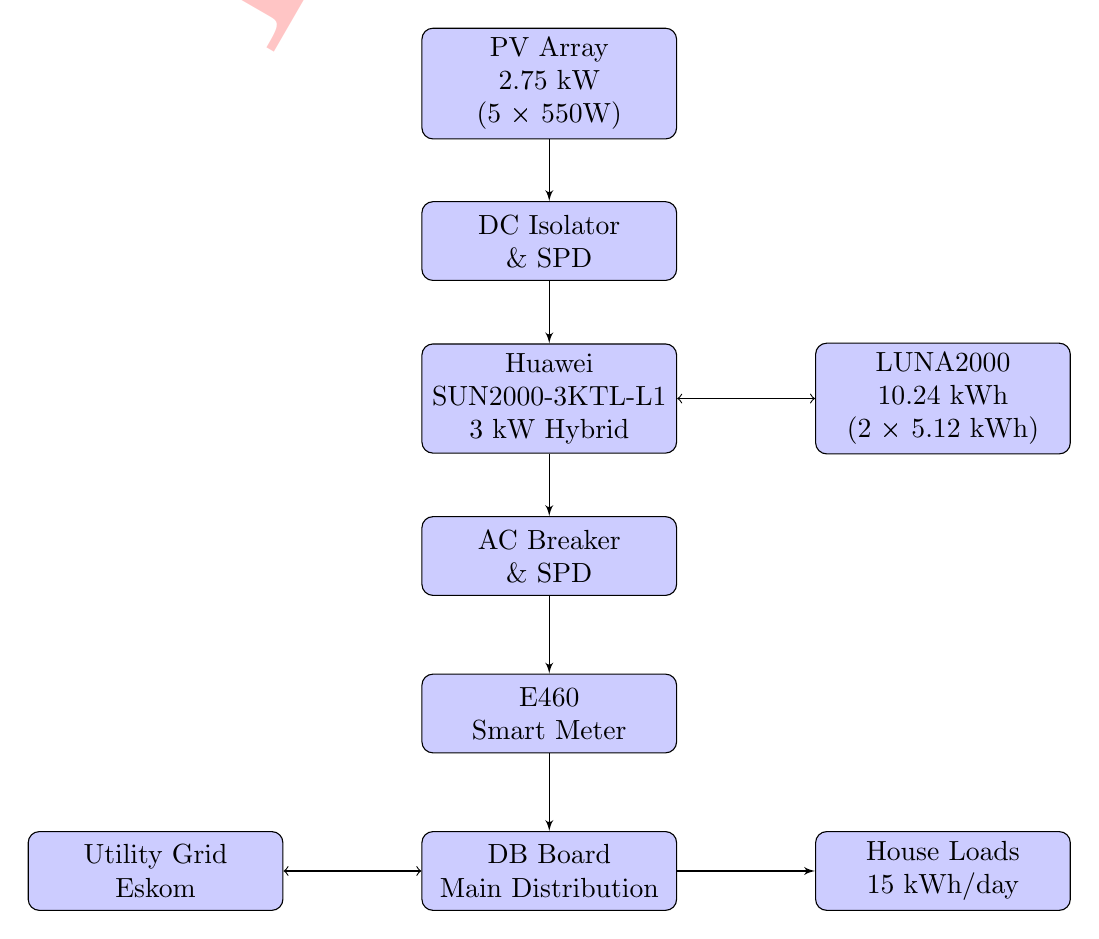
\begin{tikzpicture}[
    node distance=2cm,
    block/.style={rectangle, draw, fill=blue!20, text width=3cm, text centered, rounded corners, minimum height=1cm},
    line/.style={draw, -latex'}
]

% PV Array
\node [block] (pv) {PV Array\\2.75 kW\\(5 × 550W)};

% DC Isolator
\node [block, below of=pv] (dcisolator) {DC Isolator\\\& SPD};

% Inverter
\node [block, below of=dcisolator] (inverter) {Huawei\\SUN2000-3KTL-L1\\3 kW Hybrid};

% Battery
\node [block, right of=inverter, xshift=3cm] (battery) {LUNA2000\\10.24 kWh\\(2 × 5.12 kWh)};

% AC Breaker
\node [block, below of=inverter] (acbreaker) {AC Breaker\\\& SPD};

% Smart Meter
\node [block, below of=acbreaker] (meter) {E460\\Smart Meter};

% DB Board
\node [block, below of=meter] (db) {DB Board\\Main Distribution};

% Grid
\node [block, left of=db, xshift=-3cm] (grid) {Utility Grid\\Eskom};

% Loads
\node [block, right of=db, xshift=3cm] (loads) {House Loads\\15 kWh/day};

% Connections
\path [line] (pv) -- (dcisolator);
\path [line] (dcisolator) -- (inverter);
\path [line, <->] (inverter) -- (battery);
\path [line] (inverter) -- (acbreaker);
\path [line] (acbreaker) -- (meter);
\path [line] (meter) -- (db);
\path [line, <->] (db) -- (grid);
\path [line] (db) -- (loads);

\end{tikzpicture}
\end{center}

\section{Appendix B: Technical Datasheets}

\textit{[Technical datasheets for all major components would be attached here]}

\begin{itemize}
    \item JA Solar JAM72S30-550W Panel Datasheet
    \item Huawei SUN2000-3KTL-L1 Inverter Datasheet
    \item Huawei LUNA2000-5-S0 Battery Datasheet
    \item Landis+Gyr E460 Smart Meter Datasheet
\end{itemize}

\section{Appendix C: Installation Checklist}

\textit{[Detailed installation checklist would be provided here for use by installation team]}

\section{Appendix D: Commissioning Test Results}

\textit{[Template for recording test results during commissioning]}

\begin{table}[h]
\centering
\begin{tabular}{@{}p{6cm}p{3cm}p{3cm}@{}}
\toprule
\textbf{Test Parameter} & \textbf{Spec} & \textbf{Result} \\
\midrule
PV String Voltage (Voc) & 230V DC & \underline{\hspace{2cm}} \\
PV String Current (Isc) & 14A DC & \underline{\hspace{2cm}} \\
Insulation Resistance (DC+) & >1 M$\Omega$ & \underline{\hspace{2cm}} \\
Insulation Resistance (DC-) & >1 M$\Omega$ & \underline{\hspace{2cm}} \\
Earth Resistance & <10 $\Omega$ & \underline{\hspace{2cm}} \\
AC Output Voltage & 230V ±10\% & \underline{\hspace{2cm}} \\
AC Output Frequency & 50Hz ±1\% & \underline{\hspace{2cm}} \\
RCD Trip Test & <30mA & \underline{\hspace{2cm}} \\
Anti-Islanding Test & Pass & \underline{\hspace{2cm}} \\
Battery SoC & 50-100\% & \underline{\hspace{2cm}} \\
\bottomrule
\end{tabular}
\caption{Commissioning Test Template}
\end{table}

\end{document}
